\documentclass[12pt, twoside]{article}
\input{../preamble}
\usepackage{pgfplots}
\usepgfplotslibrary{fillbetween}
\pgfplotsset{compat=1.16}

\fancyhead[LE]{\thepage}
\fancyhead[RO]{Name: \hspace{4cm} \,\\ \hspace{2.9cm} \,}
\fancyhead[LO]{La Scuola d'Italia / Dr.\ Huson / IB Math \\* 31 March 2026}

\begin{document}
\subsubsection*{5.10 Classwork: Tangent Lines and Enclosed Area}

\begin{enumerate}

\item \textbf{(no calculator)} The graph of $f(x) = 4x - x^2$ and the line $L$
are shown. $L$ is tangent to the graph of $f$ at the point $P(1, 3)$.

\begin{center}
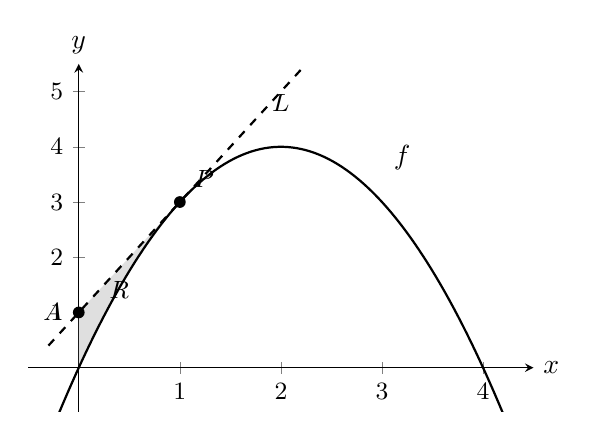
\begin{tikzpicture}
\begin{axis}[
    width=8cm, height=6cm,
    axis lines=middle,
    xlabel={$x$}, ylabel={$y$},
    xmin=-0.5, xmax=4.5,
    ymin=-0.8, ymax=5.5,
    xtick={1,2,3,4},
    ytick={1,2,3,4,5},
    tick label style={font=\small},
    every axis x label/.style={at={(ticklabel* cs:1)}, anchor=west},
    every axis y label/.style={at={(ticklabel* cs:1)}, anchor=south},
]
\addplot[name path=L, dashed, thick, domain=-0.3:2.2, samples=2] {2*x+1};
\addplot[name path=F, thick, domain=-0.2:4.2, samples=100] {4*x-x^2};
\addplot[gray!25] fill between[of=L and F, soft clip={domain=0:1}];
\node[fill=black, circle, inner sep=1.5pt, label={above right:\small $P$}] at (axis cs:1,3) {};
\node[fill=black, circle, inner sep=1.5pt, label={left:\small $A$}] at (axis cs:0,1) {};
\node at (axis cs:3.2,3.8) {$f$};
\node at (axis cs:2,4.8) {\small $L$};
\node at (axis cs:0.4,1.4) {\small $R$};
\end{axis}
\end{tikzpicture}
\end{center}

\begin{enumerate}
\item[(a)] Show that the equation of $L$ is $y = 2x + 1$. \hfill [2]
\vspace{1.5cm}
\item[(b)] $L$ meets the $y$-axis at the point $A$. Find the area of the shaded
region $R$, bounded by the graph of $f$, the line segment $AP$,
and the $y$-axis. \hfill [4]
\end{enumerate}
\vspace{1.5cm}

\newpage
\item \textbf{(no calculator)} The graph of $f(x) = e^x$ and the line $L$ are shown.
$L$ is tangent to the graph of $f$ at the point $P(1, e)$.

\begin{center}
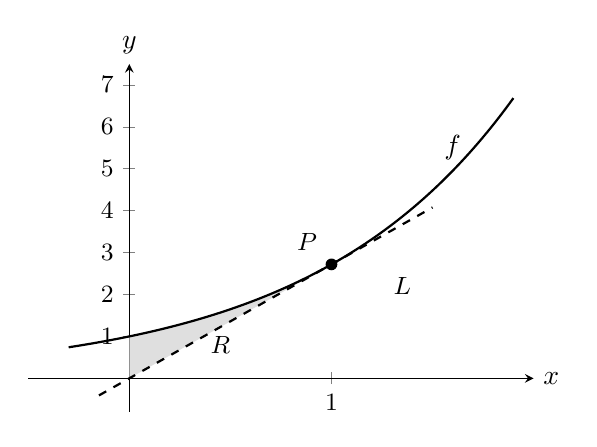
\begin{tikzpicture}
\begin{axis}[
    width=8cm, height=6cm,
    axis lines=middle,
    xlabel={$x$}, ylabel={$y$},
    xmin=-0.5, xmax=2,
    ymin=-0.8, ymax=7.5,
    xtick={1},
    ytick={1,2,...,7},
    tick label style={font=\small},
    every axis x label/.style={at={(ticklabel* cs:1)}, anchor=west},
    every axis y label/.style={at={(ticklabel* cs:1)}, anchor=south},
]
\addplot[name path=F, thick, domain=-0.3:1.9, samples=100] {exp(x)};
\addplot[name path=L, dashed, thick, domain=-0.15:1.5, samples=2] {exp(1)*x};
\addplot[gray!25] fill between[of=F and L, soft clip={domain=0:1}];
\node[fill=black, circle, inner sep=1.5pt, label={[font=\small]above left:$P$}]
    at (axis cs:1,{exp(1)}) {};
\node at (axis cs:1.6,5.5) {$f$};
\node at (axis cs:1.35,2.2) {\small $L$};
\node at (axis cs:0.45,0.8) {\small $R$};
\end{axis}
\end{tikzpicture}
\end{center}

\begin{enumerate}
\item[(a)] Write down $f'(x)$. \hfill [1]
\vspace{1cm}
\item[(b)] Show that the equation of $L$ is $y = ex$. \hfill [2]
\vspace{1.5cm}
\item[(c)] Find the area of the shaded region $R$, bounded by the graph of $f$,
the line $L$, and the $y$-axis. \hfill [4]
\end{enumerate}
\vspace{1.5cm}

\newpage
\item \textbf{(no calculator)} The graph of $f(x) = x^3$ and the line $L$ are shown.
$L$ is tangent to the graph of $f$ at the point $P(1, 1)$ and intersects the
curve again at point $Q$.

\begin{center}
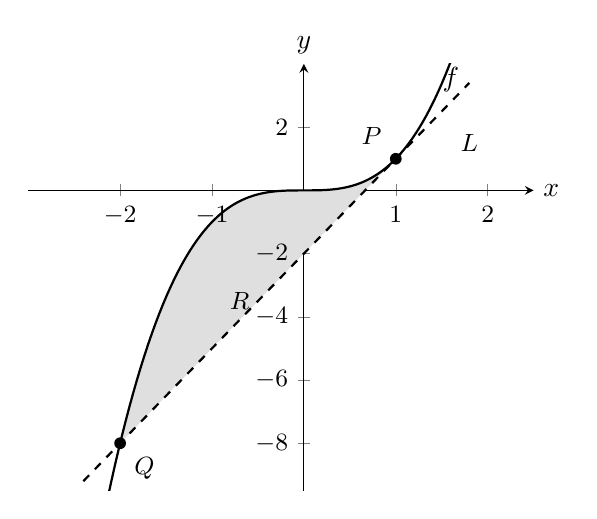
\begin{tikzpicture}
\begin{axis}[
    width=8cm, height=7cm,
    axis lines=middle,
    xlabel={$x$}, ylabel={$y$},
    xmin=-3, xmax=2.5,
    ymin=-9.5, ymax=4,
    xtick={-2,-1,1,2},
    ytick={-8,-6,-4,-2,2},
    tick label style={font=\small},
    every axis x label/.style={at={(ticklabel* cs:1)}, anchor=west},
    every axis y label/.style={at={(ticklabel* cs:1)}, anchor=south},
]
\addplot[name path=F, thick, domain=-2.3:1.7, samples=100] {x^3};
\addplot[name path=L, dashed, thick, domain=-2.4:1.8, samples=2] {3*x-2};
\addplot[gray!25] fill between[of=F and L, soft clip={domain=-2:1}];
\node[fill=black, circle, inner sep=1.5pt, label={[font=\small]above left:$P$}]
    at (axis cs:1,1) {};
\node[fill=black, circle, inner sep=1.5pt, label={[font=\small]below right:$Q$}]
    at (axis cs:-2,-8) {};
\node at (axis cs:1.6,3.5) {$f$};
\node at (axis cs:1.8,1.5) {\small $L$};
\node at (axis cs:-0.7,-3.5) {\small $R$};
\end{axis}
\end{tikzpicture}
\end{center}

\begin{enumerate}
\item[(a)] Find $f'(x)$. \hfill [1]
\vspace{1cm}
\item[(b)] Show that the equation of $L$ is $y = 3x - 2$. \hfill [2]
\vspace{1.5cm}
\item[(c)] Find the coordinates of $Q$. \hfill [3]
\vspace{2.5cm}
\item[(d)] Find the area of the shaded region $R$, enclosed between the graph
of $f$ and the line $L$. \hfill [5]
\end{enumerate}

\newpage
\item \textbf{(calculator)} The graph of $f(x) = 6e^{-0.5x}$, for $x \geq 0$,
and the line $L$ are shown. $L$ is tangent to the graph of $f$ at $A$,
where the curve meets the $y$-axis. $B$ is where $L$ crosses the $x$-axis.

\begin{center}
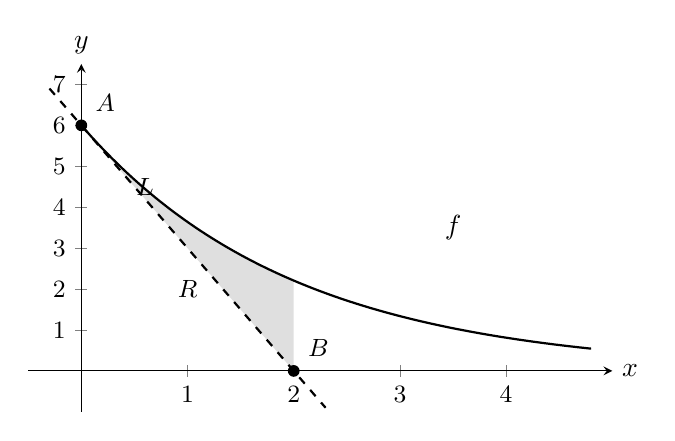
\begin{tikzpicture}
\begin{axis}[
    width=9cm, height=6cm,
    axis lines=middle,
    xlabel={$x$}, ylabel={$y$},
    xmin=-0.5, xmax=5,
    ymin=-1, ymax=7.5,
    xtick={1,2,3,4},
    ytick={1,2,...,7},
    tick label style={font=\small},
    every axis x label/.style={at={(ticklabel* cs:1)}, anchor=west},
    every axis y label/.style={at={(ticklabel* cs:1)}, anchor=south},
]
\addplot[name path=F, thick, domain=0:4.8, samples=100] {6*exp(-0.5*x)};
\addplot[name path=L, dashed, thick, domain=-0.3:2.3, samples=2] {-3*x+6};
\addplot[gray!25] fill between[of=F and L, soft clip={domain=0:2}];
\node[fill=black, circle, inner sep=1.5pt, label={[font=\small]above right:$A$}]
    at (axis cs:0,6) {};
\node[fill=black, circle, inner sep=1.5pt, label={[font=\small]above right:$B$}]
    at (axis cs:2,0) {};
\node at (axis cs:3.5,3.5) {$f$};
\node at (axis cs:0.6,4.5) {\small $L$};
\node at (axis cs:1,2) {\small $R$};
\end{axis}
\end{tikzpicture}
\end{center}

\begin{enumerate}
\item[(a)] Write down the coordinates of $A$. \hfill [1]
\vspace{1cm}
\item[(b)] Find $f'(x)$. \hfill [2]
\vspace{1.5cm}
\item[(c)] Show that the equation of $L$ is $y = -3x + 6$. \hfill [2]
\vspace{1.5cm}
\item[(d)] Find the coordinates of $B$. \hfill [1]
\vspace{1cm}
\item[(e)] Find the area of the shaded region $R$, enclosed between the graph
of $f$ and the line $L$. \hfill [4]
\end{enumerate}

\end{enumerate}
\end{document}
